% This is "sig-alternate.tex" V2.0 May 2012
% This file should be compiled with V2.5 of "sig-alternate.cls" May 2012
%
% This example file demonstrates the use of the 'sig-alternate.cls'
% V2.5 LaTeX2e document class file. It is for those submitting
% articles to ACM Conference Proceedings WHO DO NOT WISH TO
% STRICTLY ADHERE TO THE SIGS (PUBS-BOARD-ENDORSED) STYLE.
% The 'sig-alternate.cls' file will produce a similar-looking,
% albeit, 'tighter' paper resulting in, invariably, fewer pages.
%
% ----------------------------------------------------------------------------------------------------------------
% This .tex file (and associated .cls V2.5) produces:
%       1) The Permission Statement
%       2) The Conference (location) Info information
%       3) The Copyright Line with ACM data
%       4) NO page numbers
%
% as against the acm_proc_article-sp.cls file which
% DOES NOT produce 1) thru' 3) above.
%
% Using 'sig-alternate.cls' you have control, however, from within
% the source .tex file, over both the CopyrightYear
% (defaulted to 200X) and the ACM Copyright Data
% (defaulted to X-XXXXX-XX-X/XX/XX).
% e.g.
% \CopyrightYear{2007} will cause 2007 to appear in the copyright line.
% \crdata{0-12345-67-8/90/12} will cause 0-12345-67-8/90/12 to appear in the copyright line.
%
% ---------------------------------------------------------------------------------------------------------------
% This .tex source is an example which *does* use
% the .bib file (from which the .bbl file % is produced).
% REMEMBER HOWEVER: After having produced the .bbl file,
% and prior to final submission, you *NEED* to 'insert'
% your .bbl file into your source .tex file so as to provide
% ONE 'self-contained' source file.
%
% ================= IF YOU HAVE QUESTIONS =======================
% Questions regarding the SIGS styles, SIGS policies and
% procedures, Conferences etc. should be sent to
% Adrienne Griscti (griscti@acm.org)
%
% Technical questions _only_ to
% Gerald Murray (murray@hq.acm.org)
% ===============================================================
%
% For tracking purposes - this is V2.0 - May 2012

\documentclass{sig-alternate}

\begin{document}
%
% --- Author Metadata here ---
\conferenceinfo{WOODSTOCK}{'97 El Paso, Texas USA}
%\CopyrightYear{2007} % Allows default copyright year (20XX) to be over-ridden - IF NEED BE.
%\crdata{0-12345-67-8/90/01}  % Allows default copyright data (0-89791-88-6/97/05) to be over-ridden - IF NEED BE.
% --- End of Author Metadata ---

\title{Alternate {\ttlit ACM} SIG Proceedings Paper in LaTeX
Format}
%
% You need the command \numberofauthors to handle the 'placement
% and alignment' of the authors beneath the title.
%
% For aesthetic reasons, we recommend 'three authors at a time'
% i.e. three 'name/affiliation blocks' be placed beneath the title.
%
% NOTE: You are NOT restricted in how many 'rows' of
% "name/affiliations" may appear. We just ask that you restrict
% the number of 'columns' to three.
%
% Because of the available 'opening page real-estate'
% we ask you to refrain from putting more than six authors
% (two rows with three columns) beneath the article title.
% More than six makes the first-page appear very cluttered indeed.
%
% Use the \alignauthor commands to handle the names
% and affiliations for an 'aesthetic maximum' of six authors.
% Add names, affiliations, addresses for
% the seventh etc. author(s) as the argument for the
% \additionalauthors command.
% These 'additional authors' will be output/set for you
% without further effort on your part as the last section in
% the body of your article BEFORE References or any Appendices.

\numberofauthors{3} %  in this sample file, there are a *total*
% of EIGHT authors. SIX appear on the 'first-page' (for formatting
% reasons) and the remaining two appear in the \additionalauthors section.
%
\author{
% You can go ahead and credit any number of authors here,
% e.g. one 'row of three' or two rows (consisting of one row of three
% and a second row of one, two or three).
%
% The command \alignauthor (no curly braces needed) should
% precede each author name, affiliation/snail-mail address and
% e-mail address. Additionally, tag each line of
% affiliation/address with \affaddr, and tag the
% e-mail address with \email.
%
% 1st. author
\alignauthor
Johannes Spie{\ss}berger\\
% 2nd. author
\alignauthor
Ralph Hoch\\
% 3rd. author
\alignauthor 
Carola Gabriel\\
}
% There's nothing stopping you putting the seventh, eighth, etc.
% author on the opening page (as the 'third row') but we ask,
% for aesthetic reasons that you place these 'additional authors'
% in the \additional authors block, viz.
% Just remember to make sure that the TOTAL number of authors
% is the number that will appear on the first page PLUS the
% number that will appear in the \additionalauthors section.

\maketitle
\begin{abstract}
Targeted advertising is one of the key revenue sources 
for internet services. While traditional approaches tried
to suggest ads to users based on statistics derived from historical data,
modern approaches try to make use of big data.
This paper tries to give a short overview of current scientific trends 
in NoSQL and big data management. As graph databases are especially fitting for 
modelling social interactions, this paper puts an emphasis on this type of NoSql.
\end{abstract}

\terms{Big Data, targeted advertising, NoSQL, graph database}

\keywords{Big Data, targeted advertising, NoSQL, graph database}

\section{Introduction}
The recent years have shown a massive growth in data 
used for analysis in a broad range of fields.
Big data as a concept for handling this amount of information
has become a huge field for scientific research and 
business models alike. One of the cornerstones of the technical
implementation of such systems is the usage of NoSQL databases.
While these are available in many different flavours, graph based approaches
are the one that differ the most from traditional database systems.
Modelling social interactions as graphs and extracting various information
is, among other applications, one of todays key techniques for targeted advertising. TODO cite http://ieeexplore.ieee.org/stamp/stamp.jsp?tp=&arnumber=1579567
While the usage of such graph databases makes for a natural abstraction
of some real life observations, the technical implementations
of the graph database itself becomes more challenging than those of
traditional RDBMs system.
The following sections will summarize some recent research concerning 
the inner workings of graph databases.

\section{GPU based frequent graph mining}
With the availability of CUDA and opencl GPUs have become
a source of cheap computation power for significantlly less money 
than general purpose CPUs. While not applicable to all types
of computational loads, there are various fields which benefit 
immensly from a high parallelization degree TODO source.
Especially loads without the need of communication between the 
threads are well suited for GPU architectures TODO source.
The following sections will describe some applications in graph databases.

Source: http://jmlr.org/proceedings/papers/v36/kessl14.pdf
Frequent graph mining describes the search of reoccuring sub patterns 
in a set of graphs. Among various applications this technique can be used to
find similar communities within social networks TODO source.
Figure ~\ref{fig:subgraphs} shows a pattern $P$ that occurs in $G1$ and $G2$

As this problem has been shown to be NP-complete TODO source it is especially important to
find scalable algorithms to deal with this problem.
The GPU-based graph mining algorithm combines concepts from gSpan TODO source
and DMTL TODO source. 
For the effecient pruning of duplicate subgraphs the DFS-code from gSpan is used.
Parts of DMTL are used to store all isomorphisms for each pattern, which allows 
a fast computation for how many graphs in a graph database contain a certain subgraph.
In order to achieve good performance it is necessary 
to change the data structure of the graph in main memory. Hashmaps or linked lists
are not well suited for GPUs as data is not cached and therefore access locality 
must be considered for performance reasons. 
The memory layout has to happen in a way that the id and neighborhood can be quickly looked up.
To achieve this goal the combined neighborhoods of all vertices, edges and vertices are stored 
in seperate arrays. A fourth array is introduced which holds offsets to speedup the lookup between arrays.
This memory layout including the implications of how data is looked up by gSpan and DMTL allow
for a very effecient parallelization on GPUs.
For various benchmarks this technique led to significant speedups. Figure ~\ref{fig:gpuperf}
shows the performance comparison between a GPU and a sequential implementation 
for frequent graph mining on multiple datasets.
The principles of this research can also be extended to additional graph algorithms like closed graph,
maximal graph and temporal graph mining.

\begin{figure}
\centering
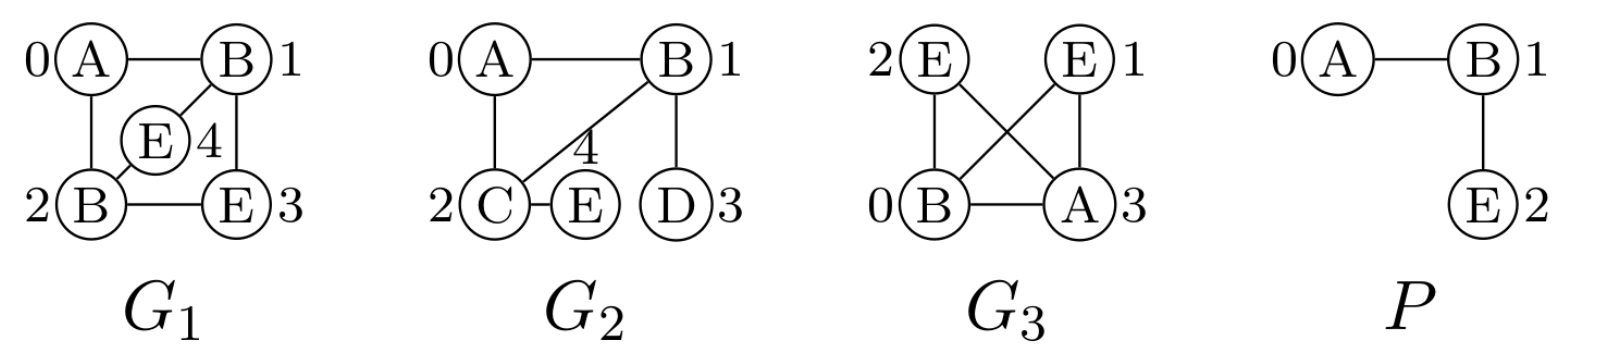
\epsfig{file=subgraphs.png, width=3in}
\caption{Graphs and pattern P}
\label{fig:subgraphs}
\end{figure}

\begin{figure*}
\centering
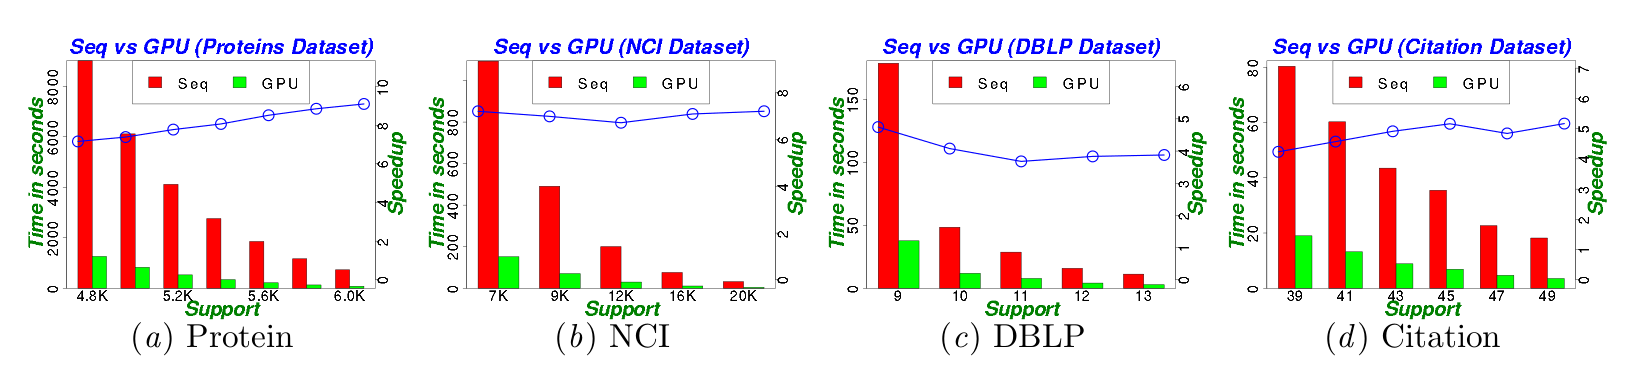
\epsfig{file=gpuperf.png, width=6in}
\caption{GPU Benchmarks}
\label{fig:gpuperf}
\end{figure*}

\section{Differential Queries}
http://ceur-ws.org/Vol-1133/paper-34.pdf
http://download.springer.com/static/pdf/593/chp%253A10.1007%252F978-3-319-10933-6_9.pdf?auth66=1422138244_54c98542c3346ab3b48752871f074418&ext=.pdf

Abandoning the rigid predefined schema of traditional database systems is one of the 
key features of NoSQL. While offering more flexibility in terms of development,
users have a hard time gaining deep knowledge of the data and its structure.
This mostly manifests in queries giving unexpected or empty result sets.
The research provided by TODO cite gives an idea of how mitigate this problem.
Diff-queries provide users with the information about which part of a query actually
matches data in the graph and which parts lead to an empty result set.
A query in a graph database can be understood as a pattern that has to match parts of the graph.
These pattern can be modeled as graphs themselfes. 
In order to be able to determine which parts of a query provide a match
and which parts will finally lead to an empty result, a common connected subgraph algorithm is
applied to the query and the graph data intself.
The resulting common subgraph can then further be used to partition 
constraints in a query into matching and non-matching conditions.

Figure ~\ref{fig:diffquery} visualizes the basic idea of
differential queries. Assume a query that searches for two soccer 
players that play for the same club and are in the same national team.
If the graph database has a player that matches parts of the query conditions,
namely playing for a national team and a club, but there is no second player with the 
same attributes, the resulting differnece graph will contain the non matching conditions.

\begin{figure*}
\centering
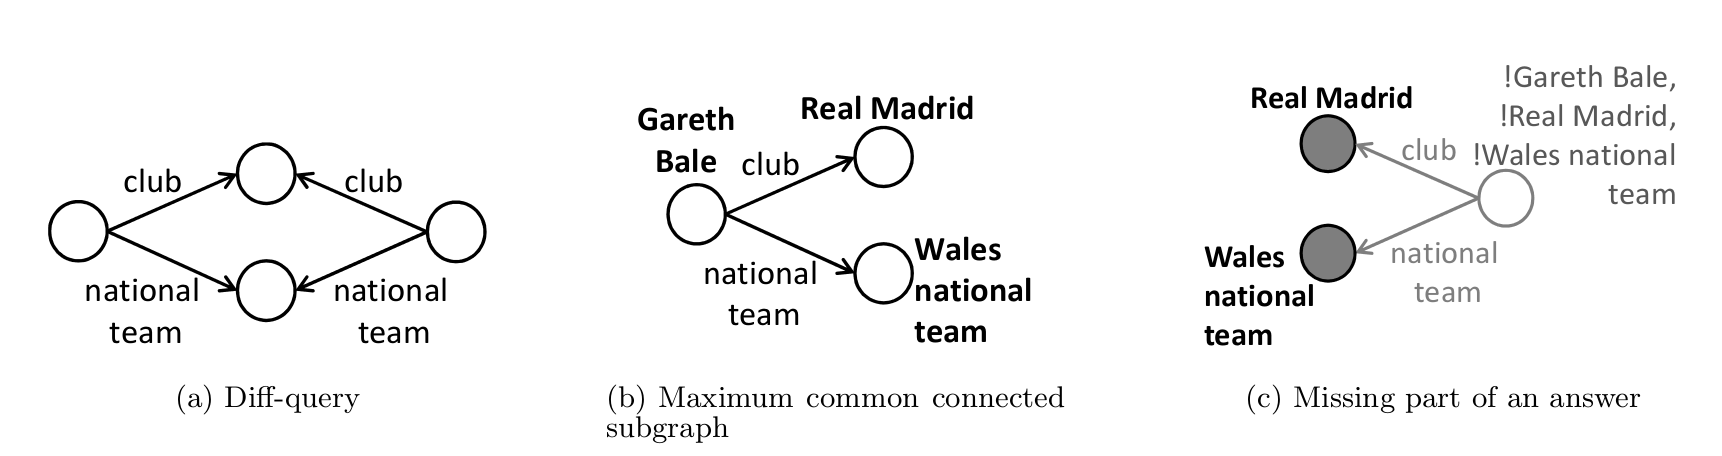
\epsfig{file=diffquery.png, width=6in}
\caption{Differential graph for data and query}
\label{fig:diffquery}
\end{figure*}


Due to the nature of these operations are large number of intermediate results 
may lead to performance problems.
This problem may be mitigated by introducing Top-K differential queries. 
While modelling the query of a graph the user is given the option to weight 
certain edges, vertices or subgraphs according to his preferences.
By using a new algorithm called relevance flooding, the specified weights are 
attached to the data in the graph database.
When calculating the maximum common subgraph, not the number matching edges and
vertices is maximized, but the score resulting from the weights given by the user.

\section{SLQ}
%https://www.cs.ucsb.edu/~xyan/papers/sigmod14_slq_demo.pdf
%http://www.vldb.org/pvldb/vol7/p565-yang.pdf
Another approach of easing the writing of graph database queries for non
professional users is the SLQ language. 
A property graph model is used for formulating queries. Aside
from having nodes and edges there are key value pairs associated with
each node. These key value pairs will be further treated as keywords.
Queries are then further transformed using a library $L$ consisting of transformations
functions. Those may include simple string replacements, semantic transformations,
numerical and topological transformations.
These functions allow for the compensation of spelling errors or the
usage of synonyms.

In an SLQ query a match in the data is derived from the mapping
of a query, including possible transformation, to the data itself. It is therefore necessary 
to define a weight for such transformations to only show the most relevant results.
As equal or predefined weighting for all transformations may not lead to an optimal 
query outcome, SLQ is able to learn and further improve the relevance of its transformations.

The first possibility is to use existing query logs of real users during an offline learning stage.
As a high quality pair of queries and their results may not always be available an online learning approach
is added. During the online operation, users can specify a number $k$ which will then be used
to display the most relevant results after applying a set of transformation. Be receiving 
feedback from the user SLQ is able to further improve the rankings of the transformations.

Figure ~\ref{fig:slqlearning} shows the basics of this learning process.

Figure ~\ref{fig:slqexample} gives an example for three possible queries and their final results.
The second query tries to find a person serving in the union army and was in a battle. By introducing 
the node Missouri the user specifies that it may be somehow related to the first conditions.

\begin{figure}
\centering
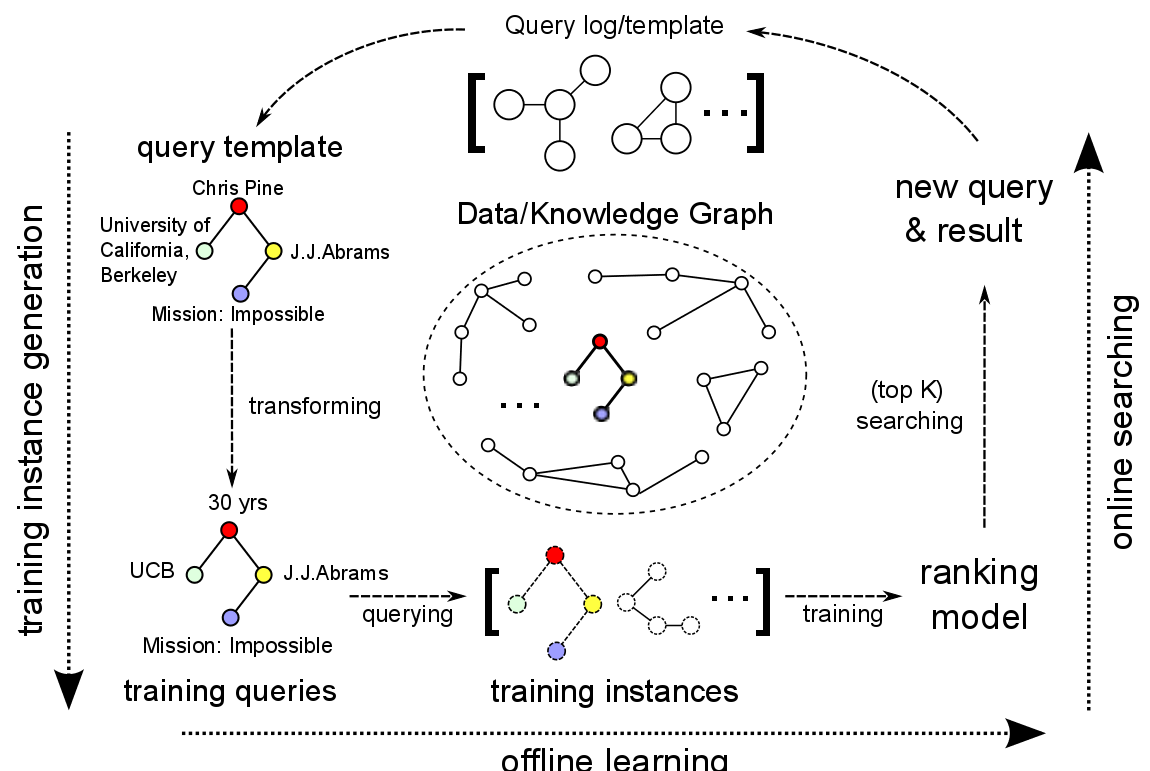
\epsfig{file=slqlearning.png, width=3in}
\caption{SLQ: graph querying framework}
\label{fig:slqlearning}
\end{figure}

\begin{figure}
\centering
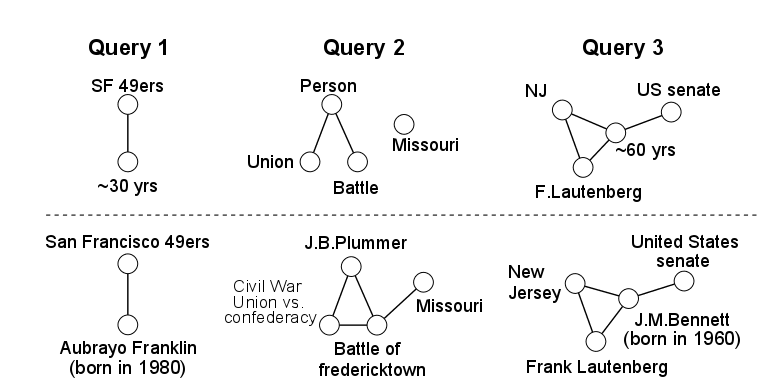
\epsfig{file=slqexample.png, width=3in}
\caption{SLQ query examples}
\label{fig:slqexample}
\end{figure}

\section{Parallel Adjacency Lists}
http://arxiv.org/pdf/1403.0701.pdf
Modelling social networks like Twitter has some particular challenges
for graph DB which come from the uneven distribution of edges between nodes.
Such graphs have the tendency to have a small number of nodes with a high number of edges
and a high number of nodes with a small number of edges. TODO zitat aus Paper 11
This makes partitioning a graph to allow for localized acces hard.
Partitioned Adjacecny Lists PAL tries to reduce the number of random accesses while minimizing the storage
space required. Edges are stored as pairs of vertices and are partitioned by a range of destination
vertices and are ordered by the source ID. These partitiones must not be of equal length but should 
be chosen such that a partition can fit into memory. This theoretically limits the number of
incoming edges a vertex may have.
As the graph connectivity is fully represented 
by the edge partitions, vertex data can be stored seperately and is partitioned 
based on the edge partitions. Retrieving verted data can be achieved by simly calculating an offset from
the edge partitions.
Edge partitions are immutable data structures and do not allow direct insertion of edges. 
To counter this problem new edges a stored in a buffer and inserted if their number exceeds a certain threshold.
During search operations these buffers are also considered.
Todo zahlen und benchmark bilder

\section{Distributed Graph Database}
%http://delivery.acm.org/10.1145/2690000/2689677/p1-dayarathna.pdf?ip=128.131.237.61&id=2689677&acc=ACTIVE%20SERVICE&key=9074CF143665B1C6.97709C79A94C9E0F.4D4702B0C3E38B35.4D4702B0C3E38B35&CFID=621086552&CFTOKEN=17755639&__acm__=1422145282_da483414101f63310da71f6d768c3e23
Current graph databases are mainly inteded to run on a single instance and therefore
face performance and availability problems. TODO Zitat aus paper 
Acadia is a distributed graph database intented to run in hybrid cloud settings.
By utilizing graph partitioning and a Master-Worker pattern it is well fit to 
operate in an environment with less than 100 workers.
Each distributed process has an associated local data store with an assigned storage quota.
When adding a new graph the partitioning happens via Hadoop and Metis and the subgraphs are then inserted into local
Neo4j instances.

\section{Conclusions}
TODO
%\end{document}  % This is where a 'short' article might terminate


%
% The following two commands are all you need in the
% initial runs of your .tex file to
% produce the bibliography for the citations in your paper.
\bibliographystyle{abbrv}
\bibliography{sigproc}  % sigproc.bib is the name of the Bibliography in this case
% You must have a proper ".bib" file
%  and remember to run:
% latex bibtex latex latex
% to resolve all references
%
% ACM needs 'a single self-contained file'!
%
%\balancecolumns % GM June 2007
% That's all folks!
\end{document}
